% Sandia National Laboratories is a multimission laboratory managed and
% operated by National Technology & Engineering Solutions of Sandia, LLC, a
% wholly owned subsidiary of Honeywell International Inc., for the U.S.
% Department of Energy’s National Nuclear Security Administration under
% contract DE-NA0003525.

% Copyright 2002-2020 National Technology & Engineering Solutions of Sandia,
% LLC (NTESS).


The syntax of this device is exactly the same as for a Current-Controlled
Current Source.  For a Current-Controlled Voltage Source just substitute an H
for the F. The H device generates a voltage, whereas the F device generates a
current.

\begin{Device}

\symbol
{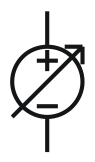
\includegraphics{ccvsSymbol}}

\device
\begin{alltt}
H<name> <(+) node> <(-) node>
+ <controlling V device name> <transresistance>
H<name> <(+) node> <(-) node> POLY(<value>)
+ <controlling V device name>*
+ < <polynomial coefficient value> >*
\end{alltt}

\examples
\begin{alltt}
HSENSE 1 2 VSENSE 10.0
HAMP 13 0 POLY(1) VIN 0 500
HNONLIN 100 101 POLY(2) VCNTRL1 VCINTRL2 0.0 13.6 0.2 0.005
\end{alltt}

\comments

In the first form, the current through a specified controlling voltage
source is multiplied by the transresistance to obtain the
voltage-source output.  The transresistance may be expressed either as
a number, a parameter, or an arbitrary brace-delimited ABM expression.

The second form using the \texttt{POLY} keyword is used in analog
behavioral modeling.  It is provided primarily for netlist
compatibility with other simulators.

H sources in any form are automatically converted within \Xyce{} to
its principal ABM device, the B nonlinear dependent source device. See
the B-source section (\ref{B_Source_Device}) and the \Xyce{} User's
Guide for more guidance on analog behavioral modeling.  For details
concerning the use of the \texttt{POLY} format, see
section~\ref{PspicePoly}.

The power supplied or dissipated by this source device is calculated
with $I \cdot \Delta V$ where the voltage drop is calculated as $(V_+ - V_-)$
and positive current flows from $V_+$ to $V_-$.  Dissipated power has a
positive sign, while supplied power has a negative sign.

H-sources were originally developed primarily to support DC and transient analysis.  
As such, their support for frequency domain analysis (AC and HB) has some limitations.  
The main limitation to be aware of is that time-dependent sources will not work with AC or HB analysis.  
These are sources in which the variable \alltt{TIME} is used in the \alltt{VALUE=} expression. 
However, this time-dependent usage is not common.  The most 
common use case is one in which the H-source is purely dependent (depends only 
on other solution variables), and this use case will work with AC and HB.  

\end{Device}
